%  !TeX  root  =  user_guide.tex

\section{Road Graph}\label{sec:roadgraph}

% when the revision of a section has been finalized,
% comment out the following line:
% \updatedisclaimer


Модуль \toolbtntwo{plugin}{Road Graph} позволяет осуществлять поиск кратчайшего
маршрута между двумя точками любого линейного векторного слоя.

\textbf{Основные возможности}:

\begin{itemize}
\item расчет маршрута, его протяженности и времени пути
\item оптимизация по критерию расстояния или времени
\item экспорт маршрута в векторный слой
\item подсветка направления движения дорог (работает медленно, чаще всего
используется в целях проверки настроек)
\end{itemize}

В качестве слоя дорог можно использовать любой линейный векторый слой в
формате, поддерживаемом QGIS. Две линии, имеющие общую точку считаются
связанными между собой. \textbf{Внимание}: при редактировании слоя дорог
в качестве СК проекта необходимо использовать СК слоя. Это вызвано тем,
что при пересчете координат между разными СК возникают погрешности, что
может приводить к появлению разрывов даже при включенном <<прилипании>>.

В атрибутивной таблице слоя могут присутсвовать и задействоваться следующие
поля:

\begin{itemize}
\item скорость движения по участку дороги "--- числовое поле
\item направление движения "--- любой тип, приводимый к строке. Прямое и
обратное направления соответствуют односторонней дороге, оба направления "---
двусторонней.
\end{itemize}

Если значение какого-либо поля не задано, или поле отсутсвует "--- используется
значение по умолчанию, изменить которое можно в настройках расширения.

\minisec{Работа с расширением}

После активации расширения в левой части окна QGIS появится еще одна панель.
Для изменения настроек модуля откройте окно \dialog{Параметры модуля RoadGraph}
из меню \mainmenuopt{Модули} \arrow \dropmenuopt{Road graph}.

\begin{figure}[ht]
    \centering
    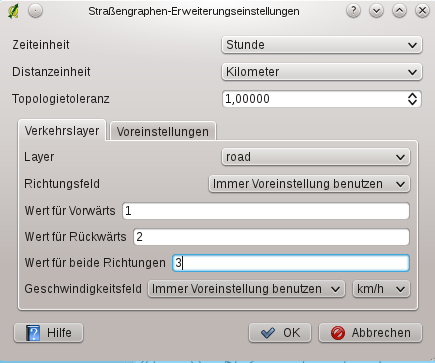
\includegraphics[clip=true, width=5cm]{roadgraph_settings}
    \caption{Настройка модуля Road Graph \nixcaption}\label{fig:roadgraphsettings}
\end{figure}

Укажите начальную и конечную точки маршрута и нажмите кнопку \button{Рассчитать}.

\begin{figure}[ht]
    \centering
    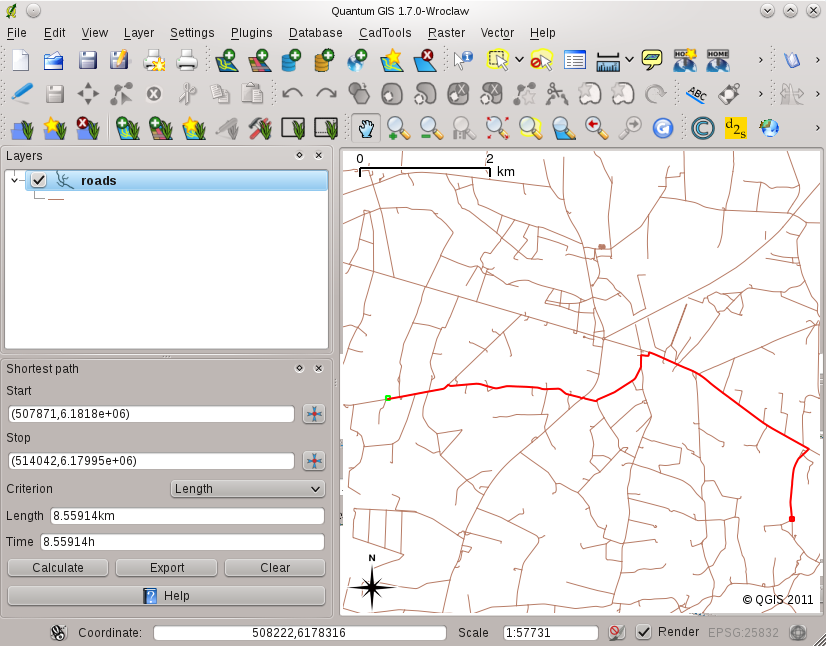
\includegraphics[clip=true, width=12cm]{roadgraph_sample}
    \caption{Модуль Road Graph \nixcaption}\label{fig:roadgraphsample}
\end{figure}

\FloatBarrier
